% Generated from master-dataset verification workflow.
% Source notebook: https://github.com/pzg8794/quantum_project/blob/gcp-main/Dynamic_Routing_Eval_Framework/notebooks/H-MABs_MasterDataset_VerificationHub.ipynb
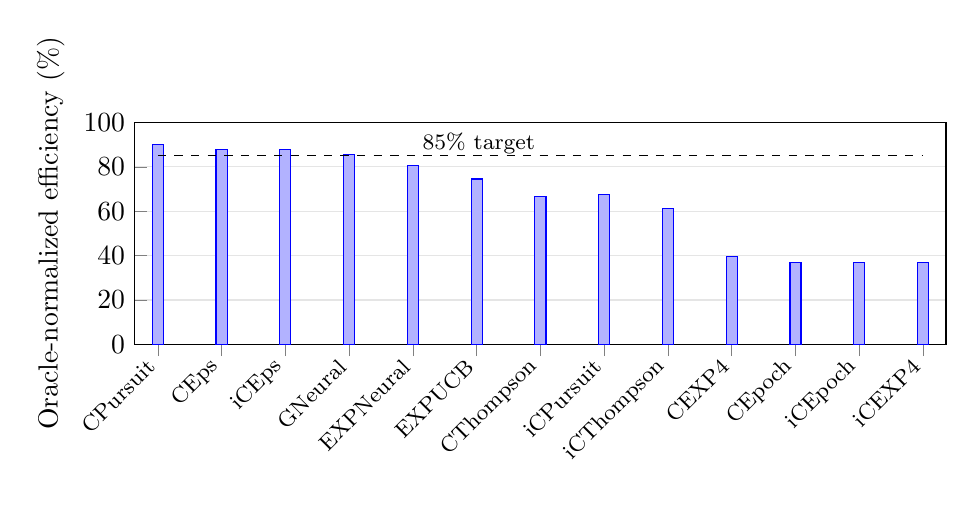
\begin{tikzpicture}
\begin{axis}[
    ybar,
    width=0.98\columnwidth,
    height=4.4cm,
    ymin=0,
    ymax=100,
    ylabel={Oracle-normalized efficiency (\%)},
    symbolic x coords={CPursuit,CEps,iCEps,GNeural,EXPNeural,EXPUCB,CThompson,iCPursuit,iCThompson,CEXP4,CEpoch,iCEpoch,iCEXP4},
    xtick=data,
    x tick label style={rotate=45,anchor=east,font=\footnotesize},
    xtick pos=bottom,
    ytick pos=left,
    ymajorgrids=true,
    grid style={draw=gray!20},
    enlarge x limits=0.03,
    bar width=4pt,
]
\addplot coordinates {
(CPursuit,89.9) (CEps,87.8) (iCEps,87.8) (GNeural,85.5) (EXPNeural,80.6) (EXPUCB,74.5) (CThompson,66.7) (iCPursuit,67.4) (iCThompson,61.1) (CEXP4,39.6) (CEpoch,37.0) (iCEpoch,37.0) (iCEXP4,37.0)
};
\addplot[sharp plot, dashed, mark=none] coordinates {(CPursuit,85) (iCEXP4,85)};
\node[font=\footnotesize, anchor=west] at (axis cs:EXPNeural,90.5) {85\% target};
\end{axis}
\end{tikzpicture}
